\documentclass[letter]{article}

\usepackage[spanish,es-nodecimaldot]{babel}
\usepackage[margin=1in]{geometry}
\usepackage{amsmath}
\usepackage{amsthm}
\usepackage{amssymb}
\usepackage{dsfont}
\usepackage[utf8]{inputenc}
\usepackage{graphicx, color}
\usepackage{algorithm}
\usepackage{algpseudocode}
\usepackage{mathrsfs}
% Cambiar el estilo de las listas
\renewcommand{\labelitemi}{$\bullet$}

% Some definitions
\floatname{algorithm}{Algoritmo}

% Author info
\title{Taller 2}
\author{Alejandro Morales Contreras$^1$}
\date{
	$^1$Departamento de Ingeniería de Sistemas, Pontificia Universidad Javeriana\\Bogotá,  Colombia \\
	\texttt{a.moralesc@javeriana.edu.co}\\~\\
	\today
}

\begin{document}
\maketitle

\tableofcontents

\section{Enunciado del problema} \label{enunciado}

Escribir e implementar un algoritmo basado en la estrategia "dividir-y-vencer" y compararlo contra su versión "iterativa". \par

El problema a trabajar es ``a partir de un número natural, calcular su representación binaria inversa". Por ejemplo, la representación binaria del número 345 es 101011001, y su representación inversa es 100110101, que es el número 309. \par

\section{Formalización del problema} \label{formalizacion}

Dado un número natural ($x \in \mathbb{N}$), su representación binaria se puede expresar así: \par

\[ x = 2^{n-1} \cdot B_1 + 2^{n-2} \cdot B_2 + \cdots + 2^{0} \cdot B_n  \]

\[ B = \left< a_i \in \left< 0, 1 \right> \right> ~|~ 1 \leq i \leq n \]

\[ b = 10^{n - 1} \cdot b_1 + 10^{n - 2} \cdot b_2 + \cdots + 10^{0} \cdot b_n \]

donde $B$ es la representación binarira en forma secuencial y $b$ es la representación binaria en decimal (base-10). Encontrar la representación binaria inversa de $x$ consistiría invertir la suma de la multiplicación de $B_i$ con las potencias de $2$ de $[n-1, 0]$ a $[0, n-1]$ así: \par

\[ y = 2^{0} \cdot B_1 + 2^{1} \cdot B_2 + \cdots + 2^{n-1} \cdot B_n \]

\subsection{Definición del problema ``representación binaria inversa''} \label{formalizacion:definicion}

El problema de hallar la representación binaria inversa de un número se define a partir de un número $x \in \mathbb{N}$, encontrar el número $y$ cuya representación binaria resulta de invertir (leer de derecha a izquierda) la representación binaria de $x$. \par

\begin{itemize}
    \item Entradas:
    \begin{itemize}
        \item $x \in \mathbb{N} ~|~ x = 2^{n-1} \cdot B_1 + 2^{n-2} \cdot B_2 + \cdots + 2^{0} \cdot B_n \land B = \left< a_i \in \left< 0, 1 \right> \right> \land 1 \leq i \leq n$
    \end{itemize}
    \item Salidas:
    \begin{itemize}
        \item $y \in \mathbb{N} ~|~ y = 2^{0} \cdot B_1 + 2^{1} \cdot B_2 + \cdots + 2^{n-1} \cdot B_n$
    \end{itemize}
\end{itemize}

\section{Algoritmos de solución} \label{algoritmos}

\subsection{Iterativo} \label{algoritmos:iterativo}

\subsubsection{Idea general de la solución} \label{algoritmos:iterativo:idea}

Convertir un número $x$ a su representación binaria puede hacerse dividiendo entre $2$ repetidamente el número, y agarrando los residuos y el último cociente para generar la representación. En la figura \ref{fig:calcular_rep_bin}, se presenta un ejemplo de este cálculo para el número $x=13$. \par

\begin{figure}[!ht]
    \centering
    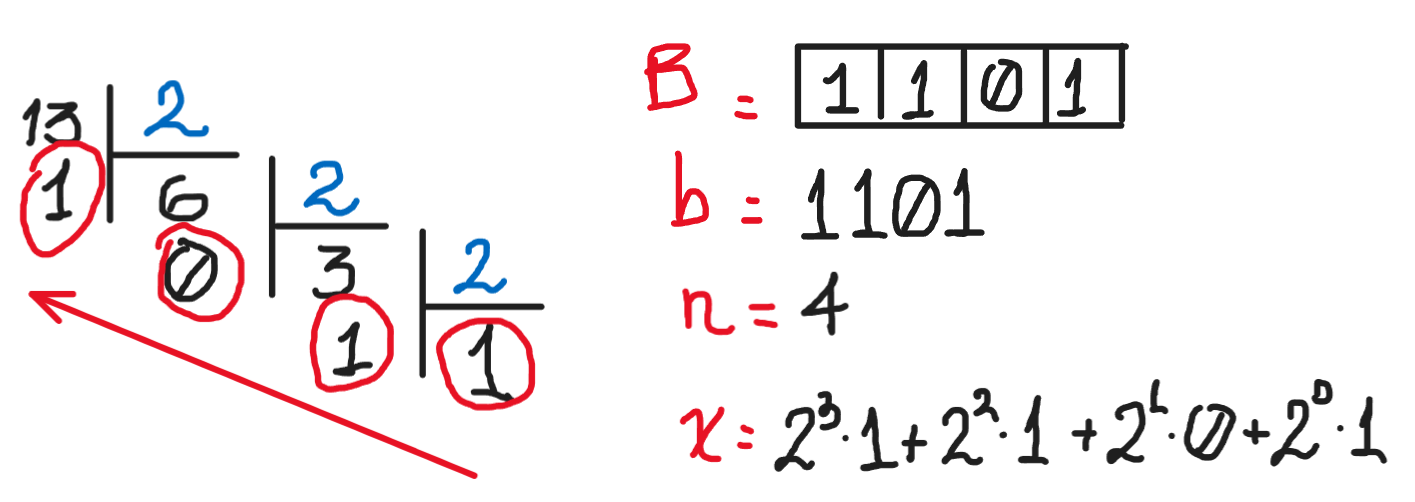
\includegraphics[scale=0.3]{img/fig1.png}
    \vspace{-1em}
    \caption{Calcular representación binaria de $x=13$}
    \label{fig:calcular_rep_bin}
\end{figure}

La representación binaria de $13$ sería entonces $1101$. Calcular la representación binaria inversa sería ahora calcular la suma de la multiplicación de los dígitos de $b$ con las potencias de $2$ desde $0$ hasta $n-1$. Para el ejemplo, podría expresarse como: \par

\[ y = 2^{0} \cdot 1 + 2^{1} \cdot 1 + 2^{2} \cdot 0  + 2^{3} \cdot 1 = 11 \]

La idea de solución consistiría entonces en dividir de dicha forma al número, guardando en un nuevo número $b$ los dígitos generados y también calculando $n$ (cantidad de dígitos). Finalmente, se extraerían los dígitos de $b$ y se calcularía la suma de potencias. \par

Para hacer esta lógica de división y residuo, se utilizarían los operadores de división entera (también expresada como división piso) y el módulo. Así mismo, el proceso truncar el último dígito de un número, así como extraerlo, se haría utilizando estos operadores con $10$ como cociente. \par

\newpage

\subsubsection{Escritura del algoritmo} \label{algoritmos:iterativo:algoritmo}

\begin{algorithm}[!ht]
\caption{Calcular representación binaria inversa de forma iterativa.}
\begin{algorithmic}[1] 
\Procedure{ReverseBinaryRepresentationIterative}{$x$}
    \State $b \leftarrow 0$
    \State $factor2 \leftarrow 1 \land factor10 \leftarrow 1$
    \While{$x > 0$}
        \State $b \leftarrow b + \Call{Mod}{x, 2} * factor10$
        \State $x \leftarrow \lfloor x \div 2 \rfloor$
        \State $factor2 \leftarrow factor2 * 2$
        \State $factor10 \leftarrow factor10 * 10$
    \EndWhile
    \State $y \leftarrow 0$
    \While{$b > 0$}
        \State $y \leftarrow y + \Call{Mod}{b, 10} * factor2$
        \State $b \leftarrow \lfloor b \div 10 \rfloor$
        \State $factor2 \leftarrow factor2 \div 2$
    \EndWhile
    \State \Return $y$
\EndProcedure
\end{algorithmic}
\end{algorithm}

\subsubsection{Análisis de complejidad} \label{algoritmos:iterativo:complejidad}

Por inspección de código: hay un solo ciclo {\it mientras-que} anidado que siempre debe durar tantas $bits$ iteraciones como tenga la representación binaria del número; entonces, este algoritmo es $O(n)$ donde $n$ es la cantidad de bits que tiene la representación binaria de $x$.

\subsubsection{Invariante} \label{algoritmos:iterativo:invariante}

Después de cada iteración, b tiene los $k$ primeros bits de la representación binaria. \par

\begin{enumerate}
    \item Inicio: $b = 0$, no se ha determinado la representación binaria.
    \item Iteración: $1 \le k < n ~|~ 0 < x$, si se supone que los $k$ primeros bits ya están en $b$, entonces la nueva iteración llevará un nuevo bit y los $k+1$ primeros bit estarán en $b$.
    \item Terminación: $b$ corresponde a los $n$ bits que son la representación binaria del número.
\end{enumerate}

\subsection{Dividir y vencer} \label{algoritmos:dividir}

\subsubsection{Idea general de la solución} \label{algoritmos:dividir:idea}

Para resolver el problema mediante un algoritmo dividir y vencer, se puede dividir el problema en tres partes: convertir el número natural en su representación binaria, invertir la representación binaria y convertir la representación binaria invertida de nuevo a número natural. Para la primera y tercera parte, se puede utilizar la misma lógica definida en la sección \ref{algoritmos:iterativo:idea}, de dividir repetidamente el número entre $2$ y ``agarrar" los residuos y el último cociente, y de hacer la suma de multiplicación de potencias $2$ con los dígitos del número invertido. \par

El problema de invertir un número (mediante un algoritmo dividir y vencer) se puede asemejar al de invertir un árbol binario. En la figura \ref{fig:invertir_arbol} se presenta un ejemplo de este ejercicio. Enfoncándose solo en los nodos hoja, se puede ver como invertir los nodos hermanos desde el nivel más profundo hacia arriba, lleva a invertir todo el árbol. \par

\begin{figure}[!ht]
    \centering
    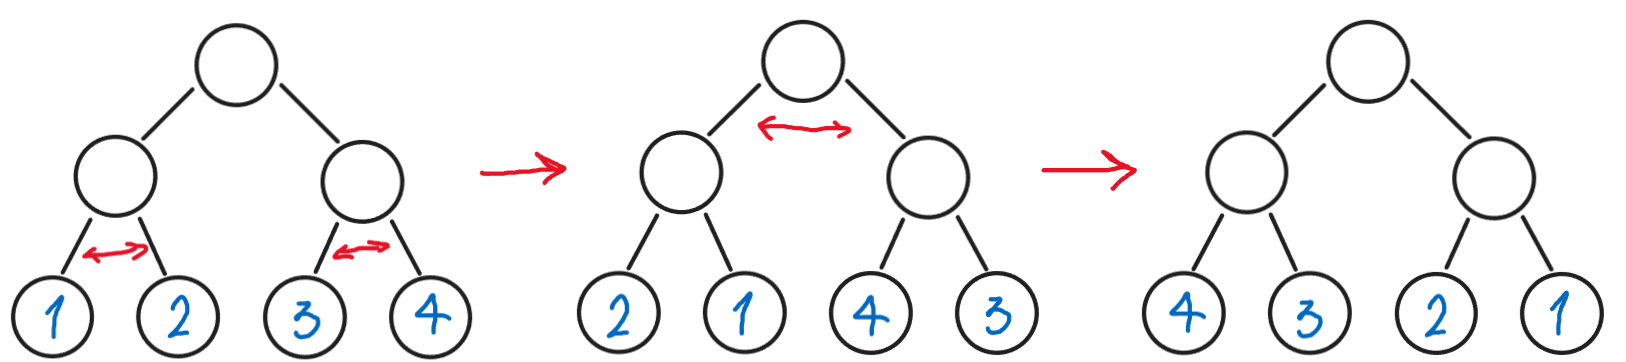
\includegraphics[scale=0.3]{img/fig2.png}
    \vspace{-1em}
    \caption{Invertir un árbol binario}
    \label{fig:invertir_arbol}
\end{figure}

Este proceso se puede asemejar al de invertir el número, donde invertir desde los grupos de $2$ elementos (y $a$ dígitos) más pequeños posibles hasta los más grandes, lleva a invertir todo el número. En la figura \ref{fig:invertir_numero} se presenta un ejemplo de este proceso.

\begin{figure}[!ht]
    \centering
    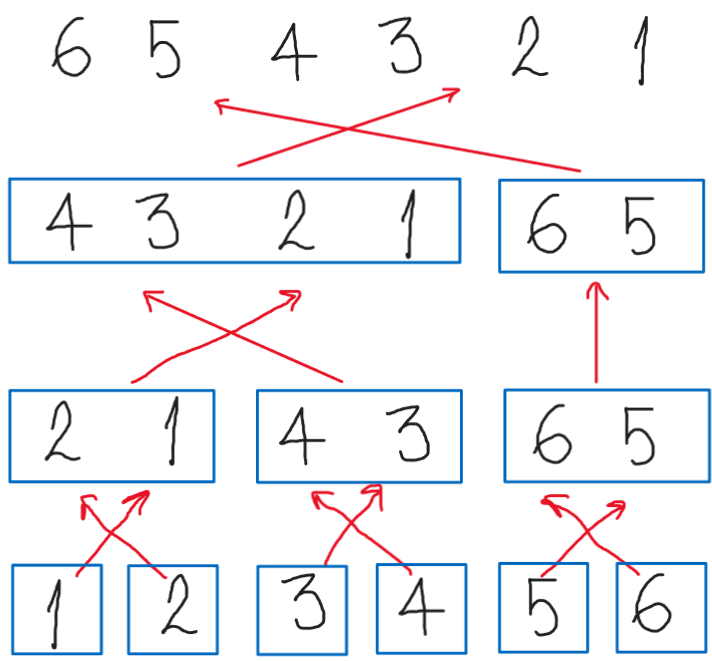
\includegraphics[scale=0.3]{img/fig3.png}
    \vspace{-1em}
    \caption{Invertir un número mediante un algoritmo dividir y vencer}
    \label{fig:invertir_numero}
\end{figure}

El proceso ahora se reduce a hallar una forma de dado un número, invertir sus dígitos desde un dígito en la posición $beg$ hasta un dígito en la posición $end$, con un pivote en la posición $q$. Una primera forma que se podría pensar, es la de utilizar una secuencia donde cada elemento es un dígito del número. Sin embargo, no hay necesidad de hacer esto si se utilizan las operaciones de truncar y reducir un número con ayuda de la división piso y módulo con cociente $10^a$.

Para demostrar esto, se asume el ejemplo de invertir los dígitos del número $123456$ con $n=6$ cantidad de dígitos, $beg=2$ dígito de inicio, $end=5$ dígito de fin y $q=3$ pivote. El resultado debería ser $145236$. Para empezar, se deben ``cortar" todos los dígitos que estén antes de $beg$ y después de $end$.

\[ num\_left = \lfloor 123456 \div 10^{6-2+1} \rfloor = 1 \]

\vspace{-1.2em}

\[ num\_right = \Call{Mod}{123456, 10^{6-5}} = 6 \]

Ahora, se calculan los dígitos que se ubican entre $beg$ y $end$ inclusive

\[ num\_mid = \Call{Mod}{\lfloor 123456 \div 10^{6-5} \rfloor, 10^{5-2+1}} = 2345 \]

Después, se dividen los dígitos de la mitad en dos grupos: los que están a la izquierda del pivote inclusive, y los que están a la derecha del pivote. \par

\[ left = \lfloor 2345 \div 10^{6 - 3 - 1} \rfloor = 23 \]

\vspace{-1.2em}

\[ right = \Call{Mod}{ 2345, 10^{6 - 3 - 1}} = 45 \]

Luego, se pasan los dígitos de la derecha a la izquierda. Esto se puede hacer fácilmente multiplicando los dígitos de la derecha por la potencia de 10 a la pivote dígitos. \par

\[ num\_mid = 45 * 10^{6 - 3 - 1} + 23 = 4523 \]

Finalmente, se unen las tres partes. \par

\[ reversed = 1 * 10^{6-2+1} + 4523 * 10^{6-5} + 6 = 145236 \]

\newpage

\subsubsection{Escritura del algoritmo} \label{algoritmos:dividir:algoritmo}

\begin{algorithm}[!ht]
\caption{Calcular representación binaria inversa de forma dividir y vencer.}
\begin{algorithmic}[1] 
\Procedure{ReverseBinaryRepresentationDC}{$x$}
    \State $b \leftarrow 0 \land n \leftarrow 0$
    \State $factor10 \leftarrow 1$
    \While{$x > 0$}
        \State $b \leftarrow b + \Call{Mod}{x, 2} * factor10$
        \State $x \leftarrow \lfloor x \div 2 \rfloor$
        \State $n \leftarrow n + 1$
        \State $factor10 \leftarrow factor10 * 10$
    \EndWhile
    \State $b2 \leftarrow \Call{ReverseNumber}{b, n, 1, n}$
    \State $y \leftarrow 0$
    \State $factor2 \leftarrow 1$
    \While{$b2 > 0$}
        \State $y \leftarrow y + \Call{Mod}{b2, 10} * factor2$
        \State $b2 \leftarrow \lfloor b2 \div 10 \rfloor$
        \State $factor2 \leftarrow factor2 * 2$
    \EndWhile
    \State \Return $y$
\EndProcedure
\end{algorithmic}
\end{algorithm}

\begin{algorithm}[!ht]
\caption{Invertir un número.}
\begin{algorithmic}[1] 
\Procedure{ReverseNumber}{$num, n, beg, end$}
    \If{$beg < end$}
        \State $q \leftarrow \lfloor (beg + end) \div 2 \rfloor$
        \State $num \leftarrow \Call{ReverseNumber}{num, n, beg, q}$
        \State $num \leftarrow \Call{ReverseNumber}{num, n, q + 1, end}$
        \State \Return $\Call{ReverseNumberAux}{num, n, beg, q, end}$
    \Else
        \State \Return $num$
    \EndIf
\EndProcedure
\end{algorithmic}
\end{algorithm}

\begin{algorithm}[!ht]
\caption{Invertir un número desde el dígito $beg$ hasta el dígito $end$ en un pivote dígito $q$.}
\begin{algorithmic}[1] 
\Procedure{ReverseNumberAux}{$num, n, beg, q, end$}
    \State $pow_1 \leftarrow \Call{Pow}{10, n - beg + 1}$
    \State $pow_2 \leftarrow \Call{Pow}{10, n - end}$
    \State $pow_3 \leftarrow \Call{Pow}{10, n - q - beg}$
    \State $num\_left \leftarrow \lfloor num \div pow_1 \rfloor$
    \State $num\_right \leftarrow  \Call{Mod}{num, pow_2}$
    \State $num\_mid \leftarrow \Call{Mod}{\lfloor num \div pow_2 \rfloor, pow1 \div pow2}$
    \State $left \leftarrow \lfloor num\_mid \div pow_3 \rfloor$
    \State $right \leftarrow \Call{Mod}{num\_mid, pow_3}$
    \State $num\_mid \leftarrow right * pow_3 + left$
    \State \Return $num\_left * pow_1 + num\_mid * pow_2 + num\_right$
\EndProcedure
\end{algorithmic}
\end{algorithm}

\subsubsection{Análisis de complejidad} \label{algoritmos:dividir:complejidad}

El algoritmo de solución consite en tres partes: la conversión del número en  binario, la inversión del número, y el posterior cálculo del numero binario invertido en decimal, $O=O_1+O_2+O_3$, en donde solo se preserva la de mayor complejidad. La complejidad de $O_1$ y $O_3$ está dada por un ciclo {\it mientras-que} que dura tantas iteraciones como {\it bits} tenga el número en su representación binaria. Entonces, estas complejidades son $O_1(n)$ y $O_3(n)$. \par

Por su parte, la inversión del número binario es un algoritmo dividir y vencer, y su complejidad puede ser expresada así y hallada a través del teorema maestro: \par

\[ T(n) = 2T(\frac{n}{2}) + O(1) \]

Utilizando las tres ecuaciones, se encuentra:

\begin{enumerate}
    \item $1 = n^{\log_b(a-\epsilon)} = n^{\log_2(2-\epsilon)} \land \epsilon = 1 \rightarrow \Theta(n^{\log_b a}) = \Theta(n)$
    \item $1 = n^{\log_ba} \log_2^kn = n^{\log_2 2} \log_2^kn \land k = ?$
    \item $1 = n^{\log_b(a-\epsilon)} = n^{\log_2(2+\epsilon)} \land \epsilon = -1$
\end{enumerate}

Por ende la complejidad de invertir el número binario es $\Theta_2(n)$. Debido a que todas las partes son equivalentes, la complejidad del algoritmo es $\Theta(n)$ donde $n$ es la cantidad de bits que tiene la representación binaria de $x$. \par

\subsubsection{Invariante} \label{algoritmos:dividir:invariante}

Después de cada llamado a $ReverseNumberAux$, el número tiene sus dígitos desde la posición $beg$ hasta $q$ y desde la posición $q+1$ hasta $end$ invertidos. \par

\section{Análisis experimental} \label{experimentos}

En esta sección se presentarán algunos los experimentos para confirmar los órdenes de complejidad de los dos algoritmos presentados en la sección \ref{algoritmos}. Así mismo, se comparará el algoritmo dividir y vencer contra el iterativo para determinar cuál se desempeña mejor. \par

\subsection{Potencias de dos}

La idea consiste en analizar las $k$ primeras potencias de $2$. Esto debido a que cada k-ésima potencia tiene $k$ bits en su representación binaria. \par

\subsubsection{Protocolo}

\begin{enumerate}
    \item Definir un número $k \in\mathbb{N}$. Se generarán las primeras $k$ potencias de $2$ desde $2^0$ hasta $2^{k-1}$.
    \item Cada algoritmo se ejecutará 10 veces con cada potencia y se guardará el tiempo promedio de ejecución.
    \item Se generan los gráficos necesarios para comparar los algoritmos.
\end{enumerate}

\newpage

\subsection{Números aleatorios}

La idea consiste en analizar $k$ números aleatorios de distinta cantidad de bits en su representación binaria. \par

\subsubsection{Protocolo}

\begin{enumerate}
    \item Definir un número $k \in\mathbb{N}$. Se generarán $k$ números aleatorios de distinta cantidad de dígitos.
    \item Cada algoritmo se ejecutará 10 veces con cada número aleatorio y se guardará el tiempo promedio de ejecución.
    \item Se compara el tiempo total promedio de ejecución de ambos algoritmos, correspondiente a la suma de los tiempos promedios de ejecución del punto 2.
\end{enumerate}

\end{document}
